\documentclass{article}
\pdfpagewidth=8.5in
\pdfpageheight=11in

\usepackage{kr}
\usepackage{times}
\usepackage{soul}
\usepackage{url}
\usepackage[hidelinks]{hyperref}
\usepackage[utf8]{inputenc}
\usepackage[small]{caption}
\usepackage{graphicx}
\usepackage{amsmath}
\usepackage{amssymb}
\usepackage{booktabs}
\usepackage[table]{xcolor}
\usepackage{multirow}
\usepackage{placeins}
\usepackage{array}
\usepackage{verbatim}
\usepackage{enumitem}
\urlstyle{same}
\definecolor{ourband}{HTML}{ECEFF3}
\definecolor{headband}{HTML}{F5F7FA}
\renewcommand{\arraystretch}{1.05}

\pdfinfo{/TemplateVersion (KR.2026.0)}

\title{ARG-Test:\\
Auditable Requirement-Driven Black-Box Test Generation\\
with Structured LLM Reasoning and Contract Verification}

\author{}

\begin{document}
\pagestyle{plain}
\pagenumbering{arabic}
\begin{titlepage}
\thispagestyle{plain}
\centering
\vspace*{\fill}
{\LARGE\bf Software Testing 42036101 Assignment 1\par}
\vspace{0.55in}
{\Large\bf Group X\par}
\vspace{0.9in}
{\large Group leader: Yi Xu (Student ID: xxxxxx)\par}
\vspace{0.18in}
{\large Group members: Luowu Zhang (Student ID: xxxxxx)\par}
\vspace{0.12in}
{\large xxx (Student ID: xxxxxx)\par}
\vspace{0.12in}
{\large xxx (Student ID: xxxxxx)\par}
\vspace{0.12in}
{\large xxx (Student ID: xxxxxx)\par}
\vspace*{\fill}
\end{titlepage}
\clearpage
\setcounter{page}{2}
\maketitle

\begin{abstract}
This report presents \textbf{ARG-Test}, an AI-enhanced black-box testing tool that converts natural-language software requirements into auditable test suites. The assignment allows either requirement documents or codebases as input; in this project we fully implement the \textbf{system-requirement-driven} branch and focus on black-box dynamic testing. The core problem is that plain large language model prompting can generate plausible test cases, but it often hides the reasoning process, misses invalid classes or boundary cases, and makes it difficult to verify whether the generated suite actually follows classical testing techniques. To address this problem, ARG-Test forces the model to produce a five-section structured testing trace consisting of \texttt{Analysis}, \texttt{Pattern}, \texttt{Steps}, \texttt{Verification}, and \texttt{FinalAnswer}, and then validates the trace using technique-specific contracts for Equivalence Partitioning, Boundary Value Analysis, Decision Table Testing, and State Transition Testing.

The final system contains a prompt builder, structured generator, parser, contract checkers, candidate reranker, repair module, exporter, and experiment scripts. We evaluate the method on an internally curated requirement dataset with \textbf{50 development requirements} and \textbf{16 held-out test requirements} covering input validation, business-rule logic, and workflow behavior. The final frozen result on the test split achieves an \textbf{average checker score of 0.959} and an \textbf{average overall coverage of 0.615}, while the best non-AI baseline reaches only \textbf{0.147} coverage and a plain LLM baseline reaches \textbf{0.030} coverage. We also run ablation and stability sanity-check experiments to understand both the strengths and the practical limitations of the approach. These results show that ARG-Test is not just a prompt, but a complete and auditable AI testing pipeline that satisfies the assignment requirements and substantially exceeds a minimal course-project implementation.
\end{abstract}

\section{Introduction}
Requirement-driven black-box testing is a meaningful testing task because many real projects start from requirement documents long before a stable codebase or executable oracle is ready. At that stage, testers still need to derive valid partitions, invalid partitions, boundary values, rule combinations, and workflow transitions from natural-language descriptions. If this early test design is weak, later implementation testing will inherit the omissions.

Large language models are attractive for this task because they can quickly read textual requirements and propose test cases. However, direct prompting is not enough for a rigorous software-testing workflow. A plain model output may look fluent while still missing illegal input classes, skipping just-below or just-above boundary points, or mixing several testing techniques without explaining why they were selected. These problems are especially serious in a course assignment that explicitly requires analysis of coverage, usefulness, and limitations rather than only a list of generated outputs.

Our solution is \textbf{ARG-Test}, a requirement-driven AI black-box testing pipeline that turns hidden reasoning into an auditable artifact. Instead of asking the model to directly output test cases in free form, ARG-Test first requires a structured testing trace. The trace is then parsed, checked, reranked, and optionally repaired before the final test suite is exported. This design follows the key philosophy of the course reference paper: reasoning should not remain opaque if we want to inspect and improve it.

This project contributes in four concrete ways. First, it defines a five-section structured testing trace for requirement-to-test generation. Second, it implements technique-aware contracts that operationalize EP, BVA, Decision Table Testing, and State Transition Testing. Third, it integrates candidate reranking and targeted repair so that the best trace is selected rather than trusting a single sample. Fourth, it provides a full experiment suite with baseline comparison, ablation, category-level generalization analysis, and a small stability sanity check. Because of this end-to-end design, the project satisfies the assignment at a level significantly above a minimal prompt-only baseline.

\section{Background and Related Concepts}
This project is grounded in four standard black-box testing techniques. \textbf{Equivalence Partitioning (EP)} divides the input space into representative valid and invalid classes. \textbf{Boundary Value Analysis (BVA)} focuses on values at, just below, and just above important limits. \textbf{Decision Table Testing} captures combinations of conditions and actions for business rules. \textbf{State Transition Testing} targets systems whose behavior depends on current state and legal or illegal transitions. These techniques are standard in software testing, but manually deriving them from natural-language requirements can be slow and inconsistent.

Traditional non-AI automation usually works only when requirement patterns are simple and explicit. For example, a rule-based script can often detect numeric ranges or mandatory fields, but it struggles when a requirement combines multiple constraints, workflow states, or implicit business logic. On the other hand, a plain LLM can read richer language, but it does not automatically provide the traceability and verification needed for a testing tool. The gap between fluency and auditability is therefore the key motivation of this work.

ARG-Test is designed to bridge that gap rather than replace classical testing concepts. The project does not invent a new testing theory. Instead, it uses AI to recover classical black-box techniques from requirements, while adding parser- and checker-based control so the result is inspectable, explainable, and experimentally analyzable.

\section{Problem Definition and Scope}
\subsection{Assignment-Compliant Problem Setting}
The assignment requires a tool that uses AI methods for software testing and accepts one of two input types: \textbf{system requirements} or \textbf{testing codebase}. Our project deliberately implements the \textbf{system-requirement input} branch. This is fully compliant with the task specification and is the most natural fit for black-box testing.

\subsection{Input, Output, and Objectives}
\textbf{Input.} The tool takes a natural-language requirement document describing a software feature, rule set, or workflow. In this project, the requirements are written in a realistic e-commerce and service-platform style.

\textbf{Output.} The tool produces five artifact layers:
\begin{enumerate}[leftmargin=1.5em]
\item A structured reasoning trace with \texttt{Analysis}, \texttt{Pattern}, \texttt{Steps}, \texttt{Verification}, and \texttt{FinalAnswer}.
\item A normalized final test suite exported as Markdown, JSON, and CSV.
\item Parser and checker artifacts for auditability.
\item Summary metrics for each requirement.
\item Aggregate experiment reports for baseline comparison, ablation, category-level generalization, and stability.
\end{enumerate}

\textbf{Objectives.} The project targets four objectives:
\begin{enumerate}[leftmargin=1.5em]
\item Generate more complete black-box test suites from requirements.
\item Make model reasoning auditable rather than opaque.
\item Compare AI and non-AI methods fairly.
\item Document AI limitations and practical mitigation steps.
\end{enumerate}

\subsection{Scope Boundaries}
The project does \textbf{not} implement a full codebase-driven white-box or static-analysis branch. It also does not claim formal semantic correctness. Instead, it aims at \textbf{auditable requirement-driven test generation} with explicit testing-technique coverage and reproducible artifacts.

\section{Method Overview}
ARG-Test uses a modular pipeline that separates generation, checking, selection, and export. The method is intentionally designed as a testing tool rather than as a single prompt.

\begin{figure*}[t]
\centering
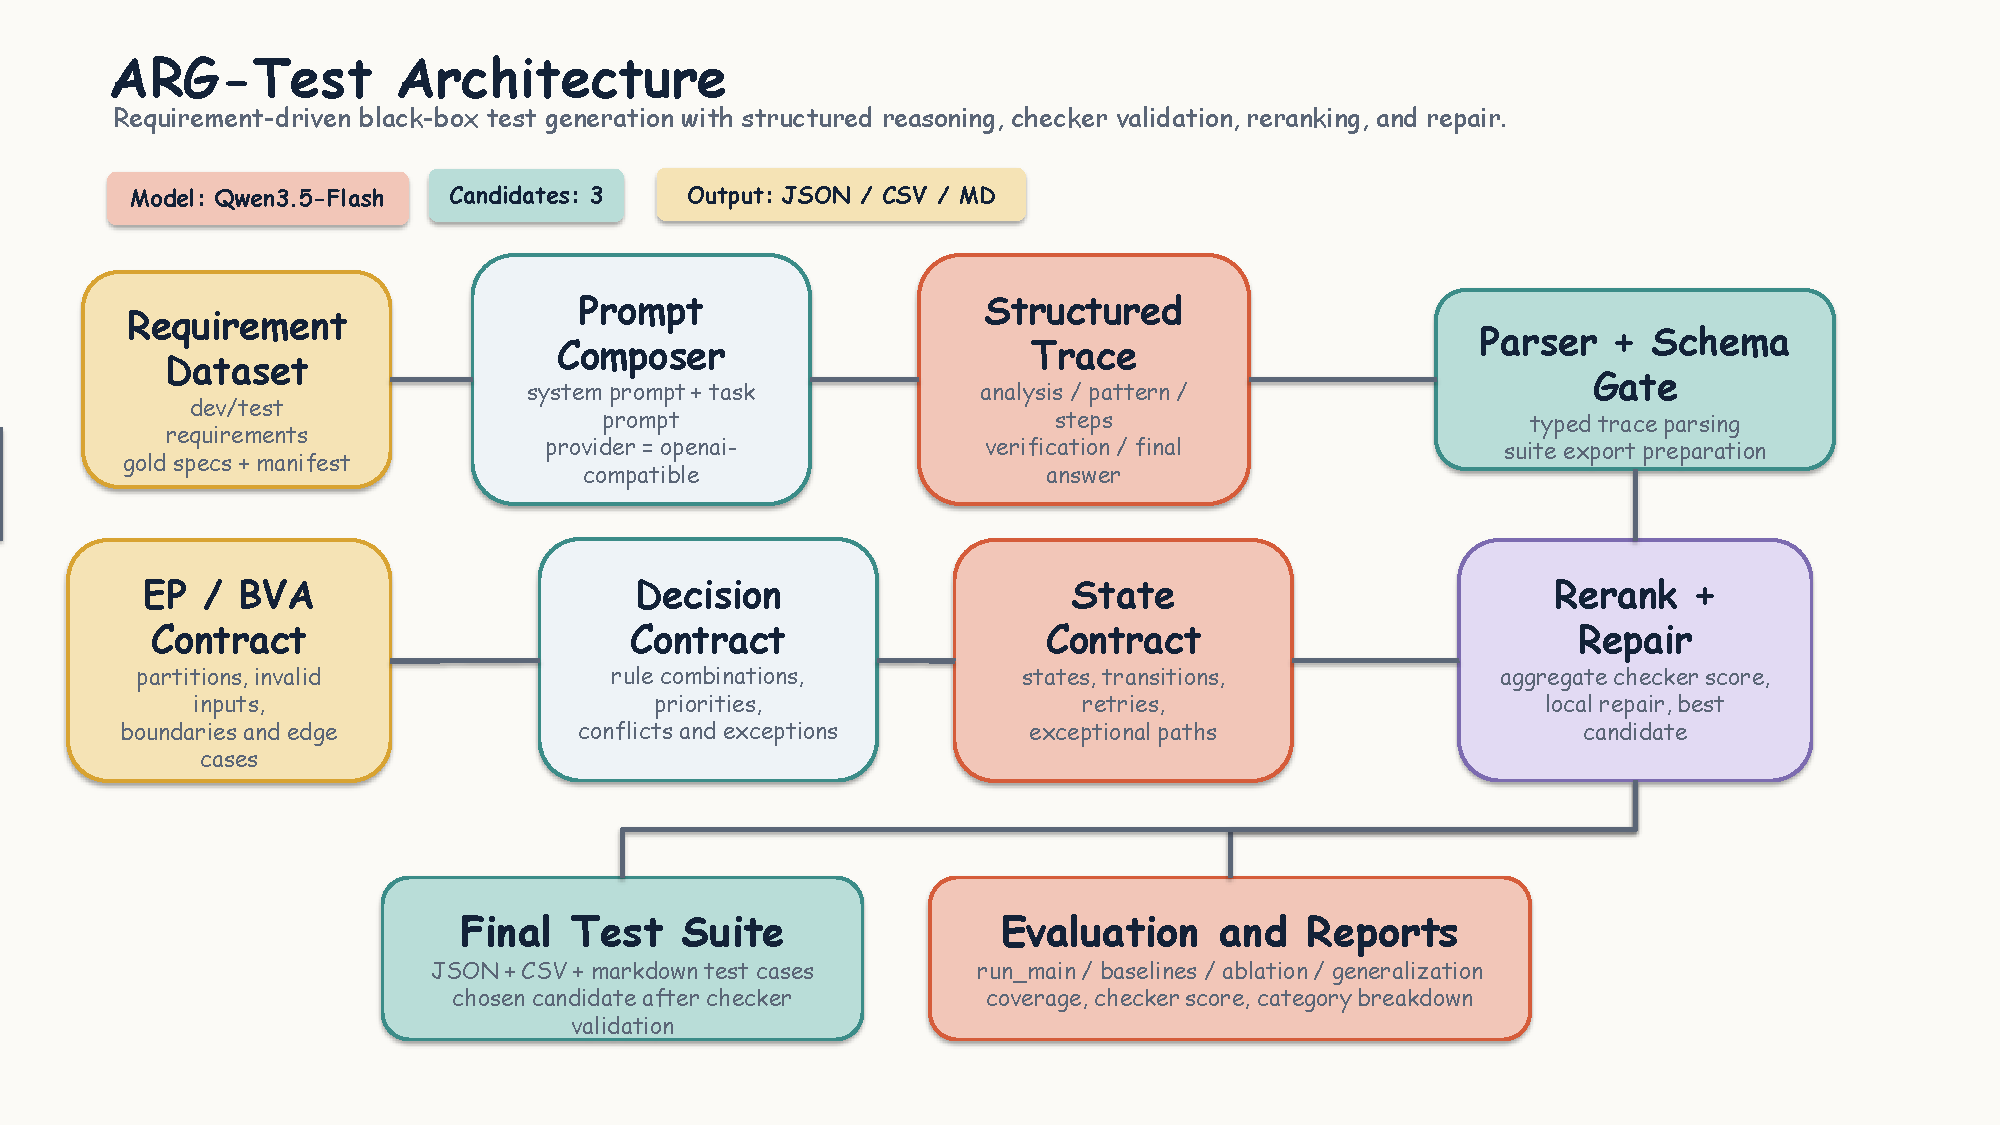
\includegraphics[width=\textwidth]{figures/arg_test_architecture_final.pdf}
\caption{The ARG-Test pipeline starts from requirement documents and gold specifications, produces multiple structured candidate traces, validates them with schema and technique-aware contracts, selects or repairs the best candidate, and exports final test artifacts together with experiment summaries.}
\label{fig:architecture}
\end{figure*}

\subsection{Structured Testing Trace}
The central representation is a five-section trace. \texttt{Analysis} extracts entities, constraints, fields, rules, states, and exceptions. \texttt{Pattern} selects black-box testing techniques and justifies why they fit the requirement. \texttt{Steps} explains how partitions, boundaries, rules, or transitions are derived. \texttt{Verification} cross-checks the trace against earlier steps. \texttt{FinalAnswer} outputs the final test-case table in a machine-readable markdown format.

This structure makes the output auditable. If the model claims to use BVA, the trace must expose which boundaries were chosen. If it claims State Transition Testing, the trace must show states, triggers, and blocked transitions. This turns hidden reasoning into a checkable interface.

\subsection{Prompting Strategy}
The prompting strategy has four layers: a system prompt, a main generation prompt, a plain-LLM baseline prompt, and a repair prompt. The system prompt enforces black-box testing and the exact five-section schema. The generation prompt injects the requirement and output template. The repair prompt preserves valid content and revises only the failed parts after checker diagnostics. The plain baseline prompt intentionally removes the structural constraints so we can measure what structure adds.

\subsection{Parser and Schema Gate}
The parser converts raw model output into a typed internal representation. This stage verifies whether the required sections exist, whether the final table is parseable, and whether required fields such as expected output are present. The parser therefore acts as the first deterministic quality gate before testing-theory contracts are applied.

\subsection{Technique-Specific Contracts}
ARG-Test implements one schema checker and four technique-aware checkers. The EP checker looks for valid and invalid partitions. The BVA checker checks lower-boundary, on-boundary, and upper-boundary style coverage. The decision checker validates rule-oriented cases and rule mapping. The state checker validates states, legal transitions, illegal transitions, and exceptional paths. These checkers do not claim full semantic proof. Their purpose is to verify whether the generated trace is consistent with the chosen testing logic.

\subsection{Candidate Reranking and Repair}
The final model output is selected from multiple candidates rather than from a single generation. Each candidate receives a score based on checker outcomes and duplicate penalties. If the best candidate still remains below the desired quality threshold, the system applies targeted repair while preserving valid test cases. This design addresses one of the main practical issues of LLM-based tools: output variance across runs.

\section{Implementation}

\subsection{Repository Modules}
\begin{table*}[t]
\centering
\small
\begin{tabular}{p{0.18\textwidth} p{0.32\textwidth} p{0.38\textwidth}}
\toprule
\textbf{Module} & \textbf{Role} & \textbf{Main Files} \\
\midrule
Prompt construction & Compose structured and baseline prompts & \texttt{prompts/}, \texttt{src/pipeline.py} \\
LLM client & Call the external model provider & \texttt{src/llm\_client.py} \\
Parser and schemas & Parse typed traces and final tables & \texttt{src/parser.py}, \texttt{src/schemas.py} \\
Checker suite & Schema, EP, BVA, decision, and state checks & \texttt{src/checker/} \\
Reranking and repair & Select best candidate and revise weak traces & \texttt{src/reranker.py}, \texttt{src/repair.py} \\
Evaluation & Compare generated suites against gold specs & \texttt{src/evaluation/metrics.py} \\
Experiment scripts & Run main, baseline, ablation, generalization, and stability workflows & \texttt{experiments/} \\
Exporter & Save JSON, CSV, markdown outputs and summary reports & \texttt{src/exporter.py} \\
\bottomrule
\end{tabular}
\caption{Main implementation modules in ARG-Test.}
\label{tab:modules}
\end{table*}

\subsection{Tool Artifact Details}
\begin{table}[h]
\centering
\small
\begin{tabular}{p{0.42\columnwidth} p{0.43\columnwidth}}
\toprule
\textbf{Item} & \textbf{Final Setting} \\
\midrule
Input type & Natural-language requirement documents \\
Testing scope & AI-enhanced black-box dynamic testing \\
Supported techniques & EP, BVA, Decision Table Testing, State Transition Testing \\
Model & Qwen3.5-Flash \\
Access path & DashScope-compatible OpenAI endpoint \\
Candidate count & 3 \\
Repair & Enabled \\
Output formats & Markdown, JSON, CSV \\
Generated artifact type & Structured traces and test cases \\
Model-generated source code & None incorporated into the tool implementation \\
\bottomrule
\end{tabular}
\caption{Final tool configuration used in the project.}
\label{tab:toolconfig}
\end{table}

The last row is important for assignment clarity. The model is used to generate \emph{testing traces and test cases}, not to write the final pipeline implementation itself. The project code remains human-authored and version-controlled.

\subsection{Prompt Artifacts}
The core prompt files are stored in the repository and included in the submission scripts package: \texttt{prompts/system\_prompt.txt}, \texttt{prompts/generation\_prompt.txt}, \texttt{prompts/repair\_prompt.txt}, and \texttt{prompts/baseline\_plain\_llm.txt}. Representative prompt snippets are included in Appendix~A.

\subsection{Exported Output Types}
For each processed requirement, ARG-Test exports raw model generations, parsed traces, checker logs, final test suites as Markdown/JSON/CSV, and per-requirement summary files. This export design directly supports the teacher's submission requirement for prompts, model settings, generated output, and experimental analysis.

\section{Experimental Setup}

\subsection{Requirement Dataset}
The dataset is an internally authored requirement collection centered on e-commerce and business-platform scenarios such as registration validation, coupon rules, refund workflows, transfer rules, payment authentication, and shipping-address validation. We use separate development and test splits.

\begin{table}[h]
\centering
\small
\begin{tabular}{lrrrr}
\toprule
\textbf{Split} & \textbf{Business} & \textbf{Input} & \textbf{Workflow} & \textbf{Total} \\
 & \textbf{Rules} & \textbf{Validation} & \textbf{State} &  \\
\midrule
Dev & 30 & 11 & 9 & 50 \\
Test & 7 & 4 & 5 & 16 \\
Total & 37 & 15 & 14 & 66 \\
\bottomrule
\end{tabular}
\caption{Dataset distribution by split and category.}
\label{tab:dataset}
\end{table}

The \texttt{dev} split is used for prompt and checker adjustment. The \texttt{test} split is frozen for final evaluation and report writing.

\subsection{Gold Specifications and Metrics}
Each requirement has a gold specification used for evaluation. Depending on the requirement type, the gold spec may contain valid partitions, invalid partitions, boundaries, decision rules, states, illegal transitions, and exception cases.

We report three primary metrics: \texttt{checker\_score}, \texttt{overall\_coverage}, and \texttt{test\_count}. We also track duplicate counts and category-level averages for generalization analysis. A key implementation detail is that non-applicable coverage dimensions are excluded rather than treated as automatic full marks. This avoids artificially inflating performance for requirements that do not involve states or decision tables.

\subsection{Baselines}
We compare ARG-Test against three baselines: (1) a rule-based non-AI generator using coarse requirement-pattern heuristics, (2) a plain LLM baseline using direct prompting without structured reasoning constraints, and (3) a structured-no-checker baseline that keeps the five-part trace but removes checker-guided selection and repair. These baselines answer different questions: whether AI beats traditional automation, whether structure helps, and whether checker-guided control adds value beyond structure alone.

\subsection{Final Execution Configuration}
The final frozen experiment used an OpenAI-compatible provider configuration with model \texttt{qwen3.5-flash}, candidate count 3, and repair enabled. The formal result root was \texttt{.local\_runs/formal\_qwen\_novpn}. The core formal workflow required approximately 246 model calls under the final settings: 150 for \texttt{dev}, 48 for \texttt{test}, 32 for baseline generation, and 16 for the final ablation refresh. A student-scale prepaid budget of 50 RMB was sufficient for the complete project workflow, including the formal run, targeted reruns, and a small stability sanity check.

\section{Results}

\subsection{Overall Scorecard}
\begin{figure}[t]
\centering
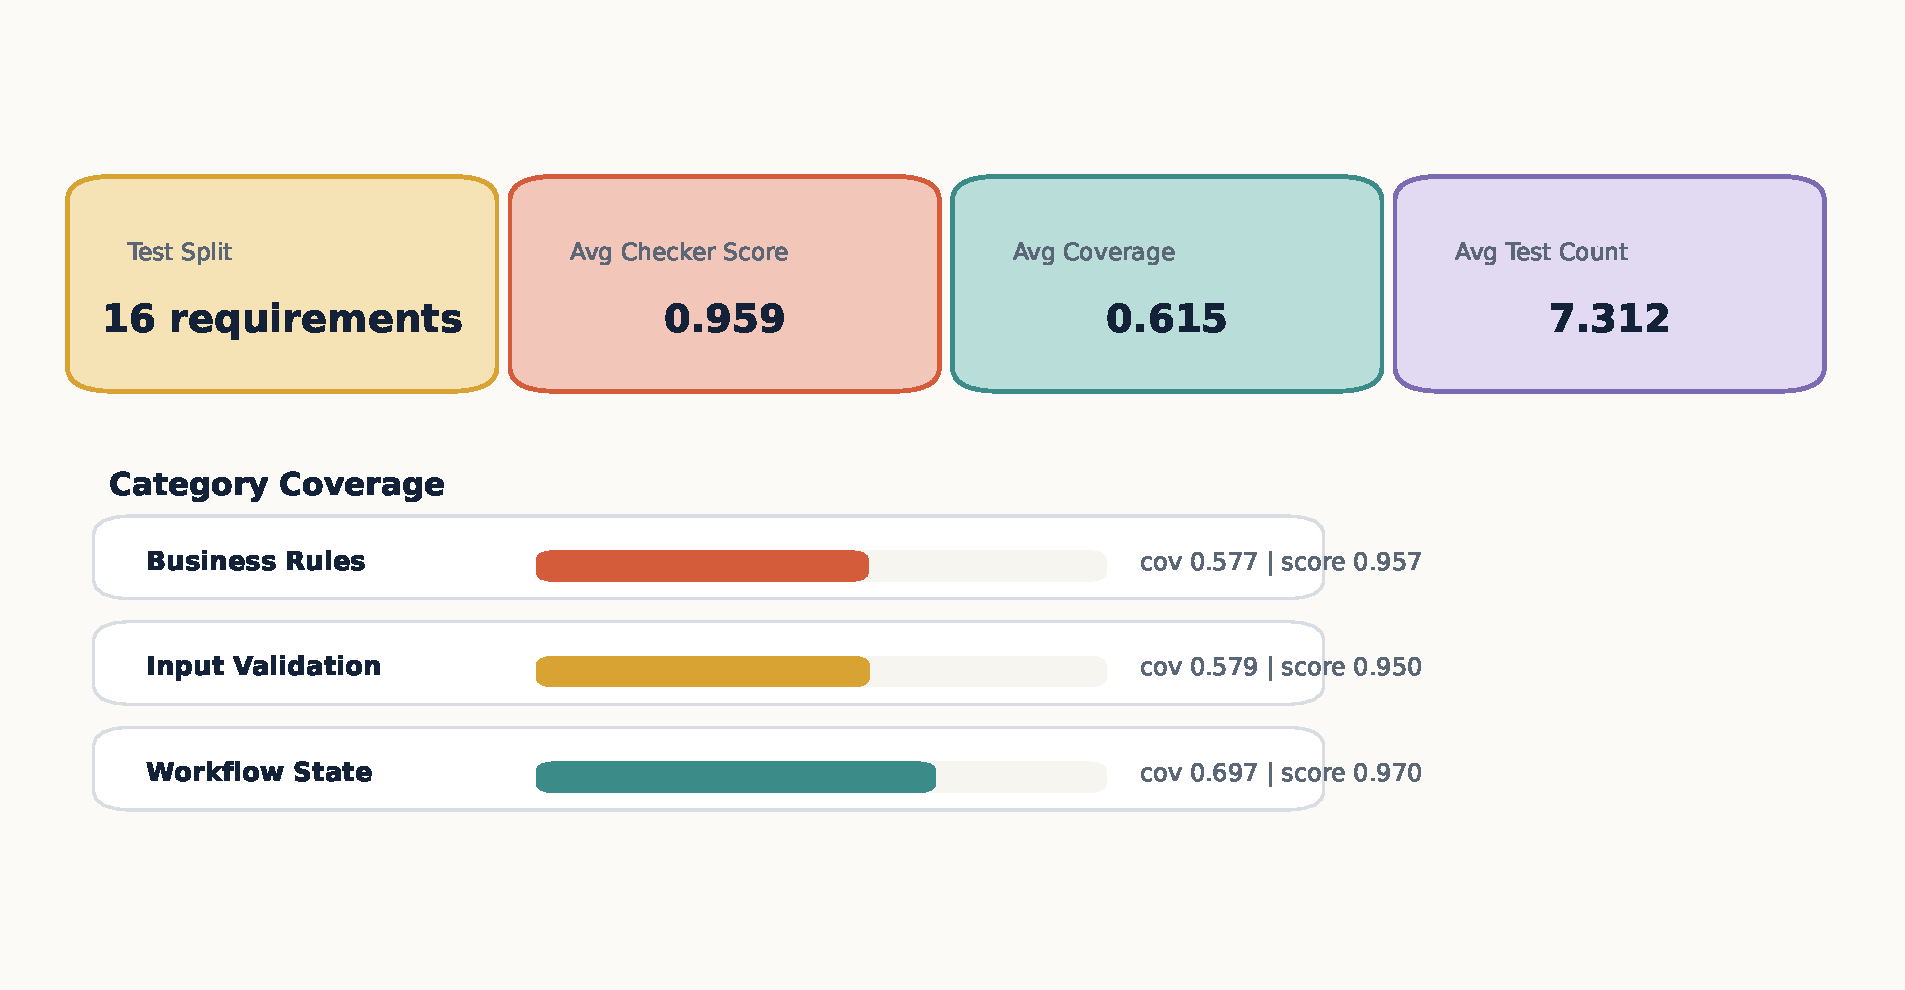
\includegraphics[width=\columnwidth]{figures/final_result_scorecard.pdf}
\caption{Compact overview of the final frozen result after targeted weak-case repair.}
\label{fig:scorecard}
\end{figure}

The final frozen test result is strong for a course project. The system processes all 16 test requirements, reaches an average checker score of 0.959, and maintains an average overall coverage of 0.615. The minimum checker score after the final weak-case promotion is 0.95, which means no remaining test requirement falls below 0.9 in checker-aligned quality.

\subsection{Main Comparison Against Baselines}
\begin{figure}[t]
\centering
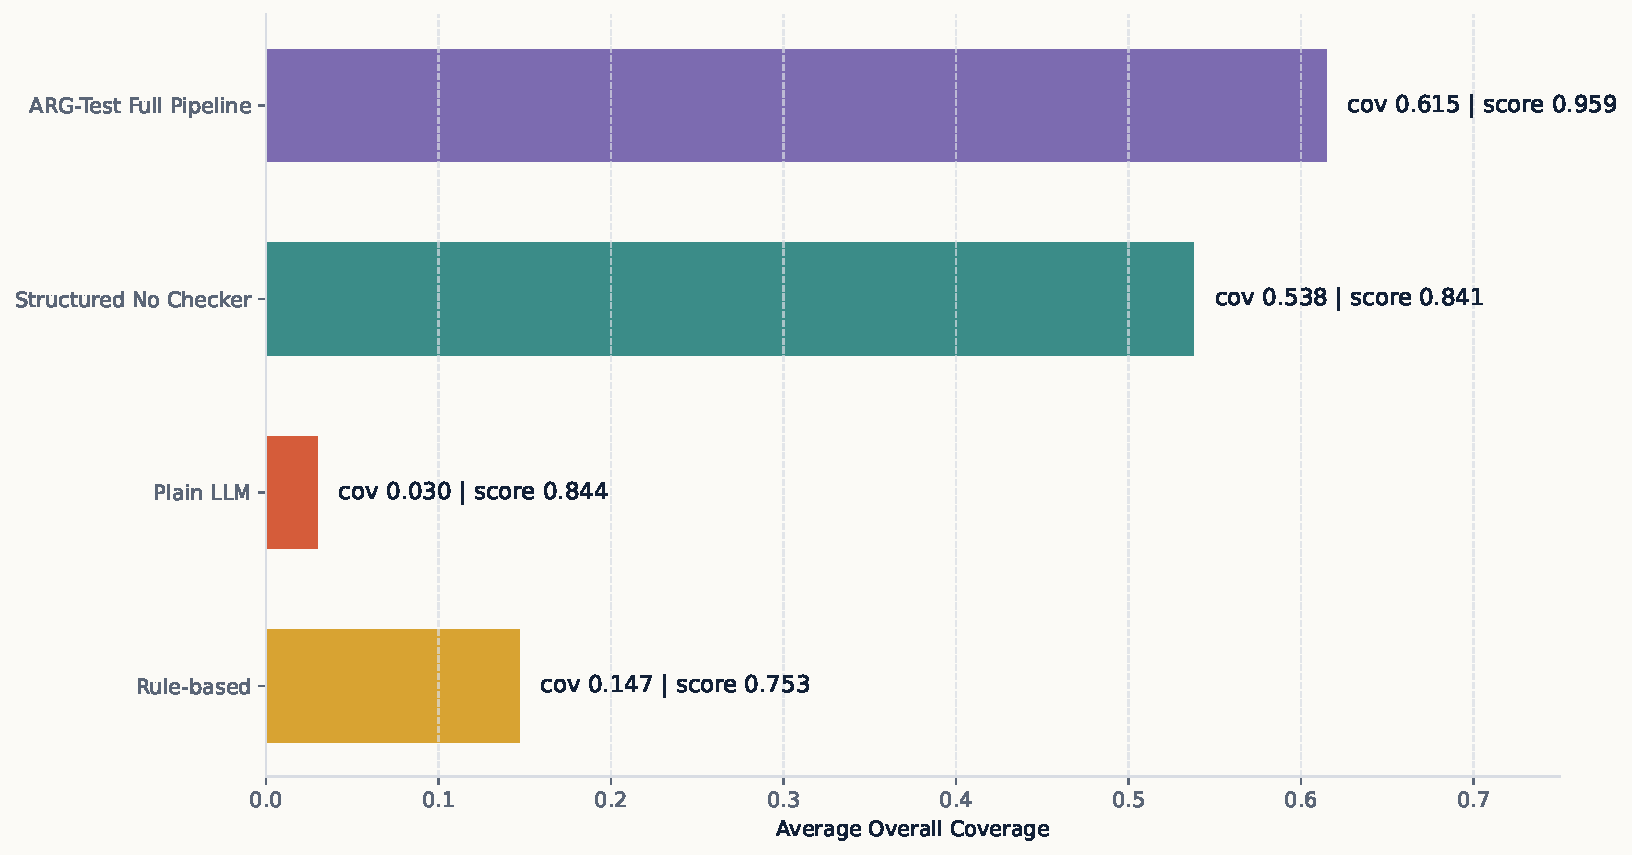
\includegraphics[width=\columnwidth]{figures/main_vs_baselines.pdf}
\caption{ARG-Test substantially improves coverage over rule-based and plain-LLM baselines, while also outperforming the structured-no-checker baseline from the standardized baseline run.}
\label{fig:mainvsbase}
\end{figure}

\begin{table*}[t]
\centering
\small
\begin{tabular}{lccc}
\toprule
\textbf{Method} & \textbf{AI-based} & \textbf{Avg Checker Score} & \textbf{Avg Overall Coverage} \\
\midrule
Rule-based & No & 0.753 & 0.147 \\
Plain LLM & Yes & 0.844 & 0.030 \\
Structured No Checker & Yes & 0.841 & 0.538 \\
\textbf{ARG-Test Full Pipeline} & \textbf{Yes} & \textbf{0.959} & \textbf{0.615} \\
\bottomrule
\end{tabular}
\caption{Main comparison on the frozen test split. The corresponding average test counts are 4.125, 7.250, 6.312, and 7.312.}
\label{tab:maincomparison}
\end{table*}

This comparison supports three conclusions. First, the full pipeline is clearly better than the non-AI rule-based baseline in coverage. Second, plain LLM prompting performs poorly in coverage even though it can produce many test cases; fluency alone is not enough. Third, the full ARG-Test pipeline also improves over the standardized structured-no-checker baseline, which shows that checker-guided control matters in practice. In relative terms, the full pipeline achieves more than four times the coverage of the rule-based baseline and more than twenty times the coverage of the plain LLM baseline.

\subsection{Generalization Across Requirement Categories}
\begin{figure}[t]
\centering
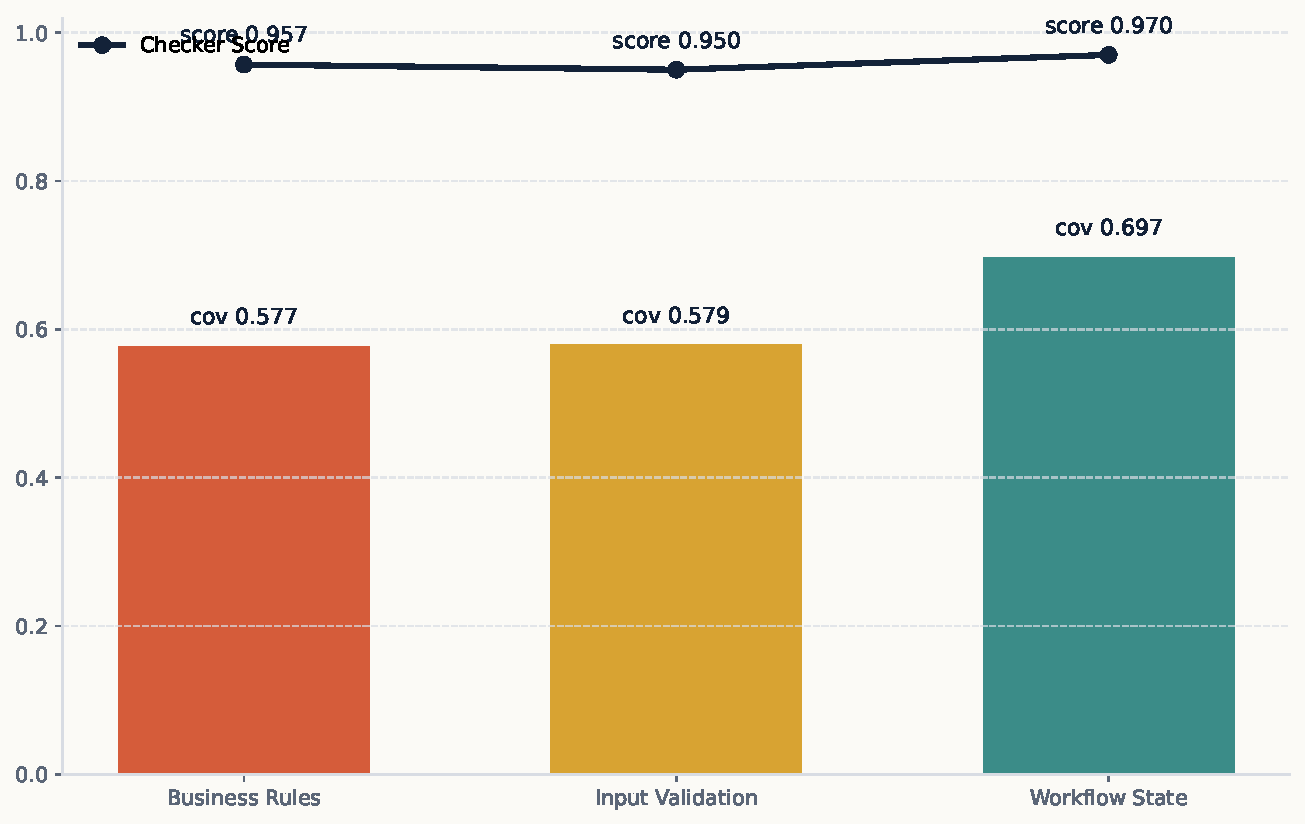
\includegraphics[width=\columnwidth]{figures/generalization_by_category.pdf}
\caption{The full pipeline remains effective across business-rule, input-validation, and workflow-state requirements.}
\label{fig:generalization}
\end{figure}

\begin{table}[h]
\centering
\small
\begin{tabular}{lccc}
\toprule
\textbf{Category} & \textbf{Count} & \textbf{Avg Score} & \textbf{Avg Coverage} \\
\midrule
Business Rules & 7 & 0.957 & 0.577 \\
Input Validation & 4 & 0.950 & 0.579 \\
Workflow State & 5 & 0.970 & 0.697 \\
\bottomrule
\end{tabular}
\caption{Category-level generalization on the frozen test split. Average test counts are 7.714, 8.500, and 5.800 respectively.}
\label{tab:generalization}
\end{table}

These results show that the system does not only work on one convenient category. Workflow-state requirements are the strongest category, which is consistent with the fact that explicit states and transition triggers are often easier to recover from text than open-ended formatting or business-rule exceptions. At the same time, both business-rule and input-validation requirements remain solid, with coverage around 0.58 and checker scores near 0.95.

\subsection{Ablation}
\begin{figure}[t]
\centering
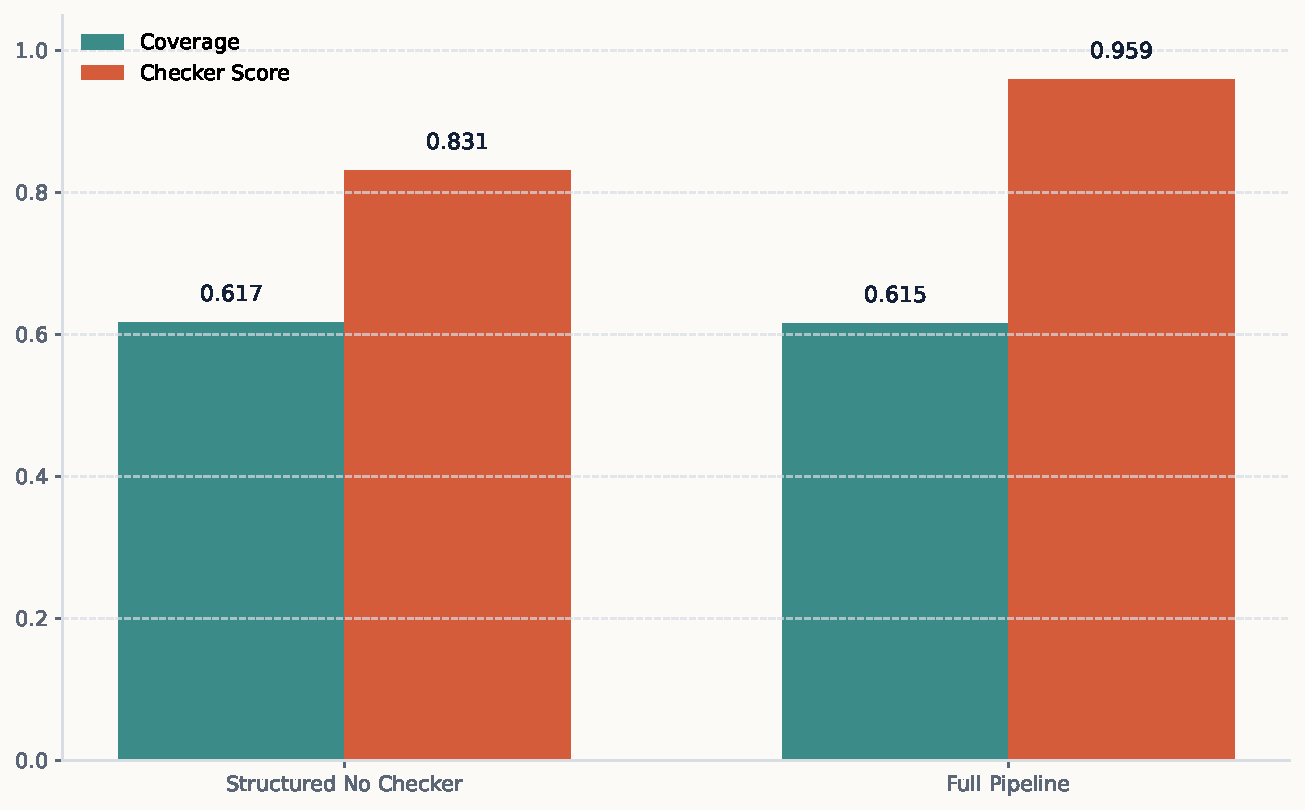
\includegraphics[width=\columnwidth]{figures/ablation_gain.pdf}
\caption{Checker-guided selection and repair strongly improve checker-aligned quality while preserving coverage at a comparable level.}
\label{fig:ablation}
\end{figure}

\begin{table}[h]
\centering
\footnotesize
\setlength{\tabcolsep}{4pt}
\resizebox{\columnwidth}{!}{%
\begin{tabular}{p{0.34\columnwidth}ccc}
\toprule
\textbf{Variant} & \textbf{Avg Score} & \textbf{Avg Coverage} & \textbf{Avg Test Count} \\
\midrule
Structured No Checker & 0.831 & 0.617 & 7.375 \\
\textbf{Full Pipeline} & \textbf{0.959} & \textbf{0.615} & \textbf{7.312} \\
\bottomrule
\end{tabular}
}
\caption{Ablation using the refreshed formal directory.}
\label{tab:ablation}
\end{table}

The ablation result is instructive. In this refreshed run, the no-checker variant reaches very similar coverage to the full pipeline, but its checker score is much lower. The full pipeline is slightly lower in average coverage and test count because reranking and repair prune weak, redundant, or loosely justified cases instead of optimizing for suite size alone. The gap is very small, while the quality gain is large: checker score increases from 0.831 to 0.959, average coverage changes only from 0.617 to 0.615, and average test count changes only from 7.375 to 7.312. Table~\ref{tab:ablation} therefore should not be read as a regression table. It shows a quality-control tradeoff in which the final pipeline gives up a negligible amount of breadth for much stronger contract consistency. The structured-no-checker row here also differs from Table~\ref{tab:maincomparison} because Table~\ref{tab:maincomparison} uses the standardized baseline run, whereas Table~\ref{tab:ablation} uses the dedicated ablation rerun. This means the checker and repair stages do not merely inflate the suite length; they improve structure, consistency, and contract alignment. The honest conclusion is therefore not that checker-guided control always increases raw coverage, but that it substantially improves quality while preserving competitive coverage.

\subsection{Stability Sanity Check}
\begin{figure}[t]
\centering
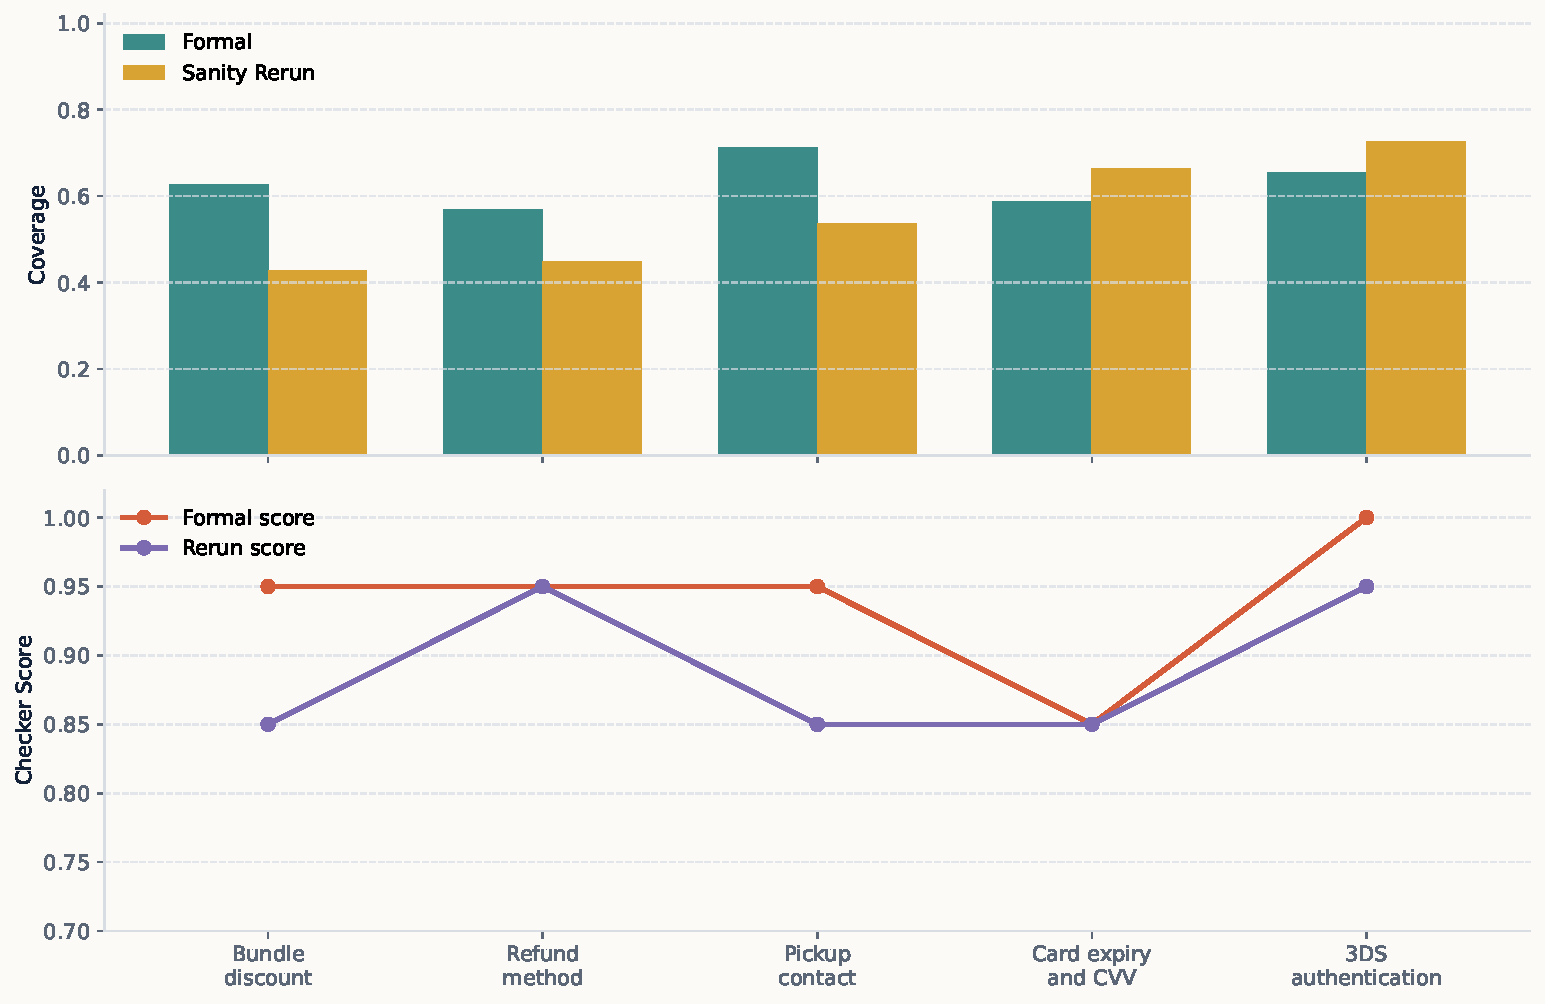
\includegraphics[width=\columnwidth]{figures/stability_sanity_check.pdf}
\caption{A five-case sanity rerun reveals some stochastic variation, which is expected for LLM-based generation, but the frozen final run remains defensible.}
\label{fig:stability}
\end{figure}

\begin{table}[h]
\centering
\small
\begin{tabular}{lr}
\toprule
\textbf{Item} & \textbf{Value} \\
\midrule
Sample size & 5 requirements \\
Strictly stable cases & 2 / 5 \\
Formal avg score & 0.940 \\
Rerun avg score & 0.890 \\
Formal avg coverage & 0.630 \\
Rerun avg coverage & 0.561 \\
Avg absolute score delta & 0.050 \\
Avg absolute coverage delta & 0.129 \\
\bottomrule
\end{tabular}
\caption{Stability sanity check on five representative requirements.}
\label{tab:stability}
\end{table}

The sanity rerun confirms that the system has some stochastic variation, which is typical for LLM-based generation. This is exactly why ARG-Test uses multiple candidates, checker-guided selection, and targeted repair. The stability experiment therefore does not weaken the project; instead, it provides honest evidence that the system needs control mechanisms and that the final frozen run should be treated as a managed evaluation artifact rather than as a deterministic oracle.

\subsection{Targeted Weak-Case Repair}
After the first formal freeze, two requirements still looked weaker than the rest: \texttt{address\_international\_format\_validation} and \texttt{payment\_card\_expiry\_and\_cvv\_validation}. We therefore performed a strictly limited targeted rerun on these cases only and promoted the better versions back into the formal directory.

This extra step improved the final quality noticeably: no requirement remains below 0.9 in checker score, only one requirement remains below 0.4 in coverage, and the remaining low-coverage case is \texttt{address\_international\_format\_validation} with 0.392 coverage. This remaining weak case is still understandable because the requirement mixes country-dependent postal-code constraints with international phone formatting, which makes the input space more open-ended than finite-state or tightly bounded business-rule scenarios.

\subsection{Representative Case Study}
\begin{figure*}[t]
\centering
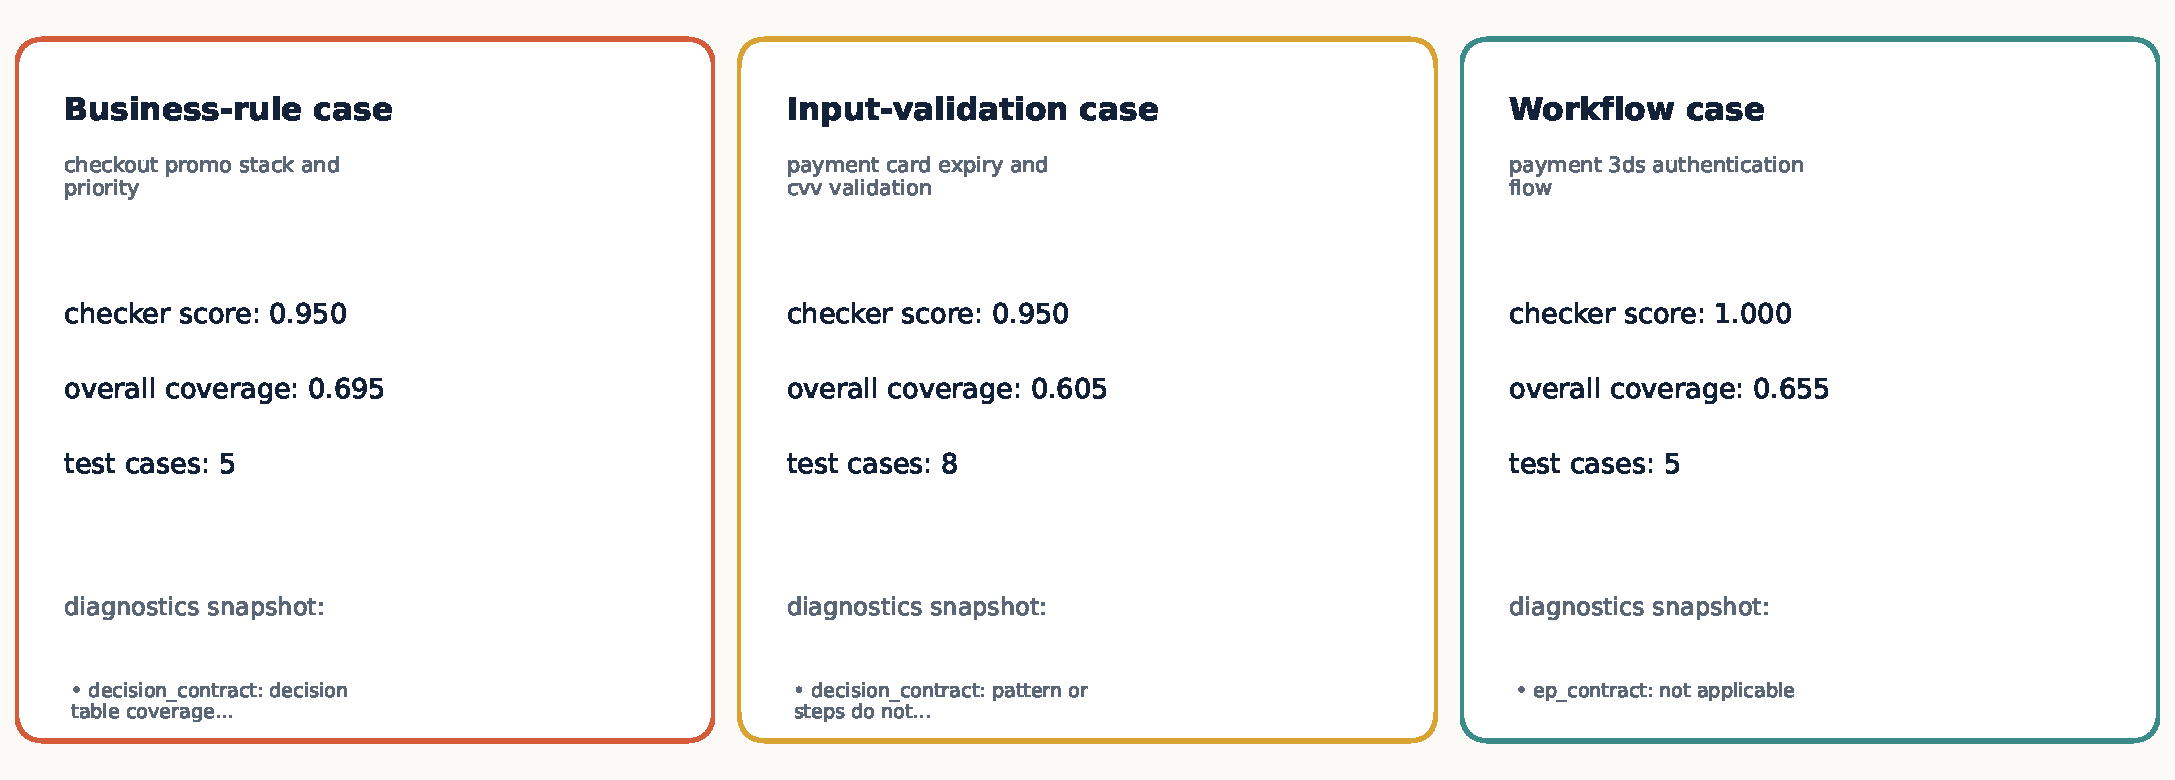
\includegraphics[width=\textwidth]{figures/case_study_snapshots.pdf}
\caption{Representative examples from business-rule, input-validation, and workflow-state settings.}
\label{fig:casestudy}
\end{figure*}

The case-study figure highlights three useful examples: \texttt{checkout\_promo\_stack\_and\_priority} as a business-rule case, \texttt{payment\_card\_expiry\_and\_cvv\_validation} as an input-validation case, and \texttt{payment\_3ds\_authentication\_flow} as a workflow-state case. These examples were chosen because together they show that the same pipeline can handle condition priority, formatted inputs, and stateful payment behavior. This category breadth is one of the strongest practical signals that the project generalizes within the chosen task scope.

\section{Comparison with a Traditional Non-AI Technique}
The assignment explicitly requires comparison with a traditional non-AI technique, and our rule-based baseline serves exactly that role.

\begin{table*}[t]
\centering
\small
\begin{tabular}{p{0.18\textwidth} p{0.31\textwidth} p{0.31\textwidth}}
\toprule
\textbf{Aspect} & \textbf{Traditional Rule-Based Baseline} & \textbf{ARG-Test Full Pipeline} \\
\midrule
Core mechanism & Deterministic pattern rules & LLM generation plus parser, checker, reranking, and repair \\
Language flexibility & Weak on implicit logic and mixed constraints & Strong on natural-language interpretation \\
Auditability & High for covered rules, low for missing rules & High due to structured trace and checker logs \\
Cost & Very low & Moderate API cost \\
Variance & Deterministic & Stochastic but controllable \\
Coverage on frozen test split & 0.147 & 0.615 \\
Best use case & Simple numeric or mandatory-field rules & Complex textual requirements with mixed logic \\
\bottomrule
\end{tabular}
\caption{Traditional non-AI rule-based baseline versus ARG-Test.}
\label{tab:nonai}
\end{table*}

This comparison shows why an AI-enhanced approach is worthwhile. The rule-based baseline is deterministic and cheap, which is attractive, but it cannot recover enough information from realistic natural-language requirements. ARG-Test is more expensive and more complex, yet it provides much stronger coverage and richer artifacts. For the assignment, this trade-off is justified because the goal is not only automation, but useful AI-enhanced testing.

\section{Discussion}

\subsection{Why the Project Works}
The project works because it does not ask the model to solve the whole problem in one opaque step. Instead, it decomposes the task into three control layers. The structured trace makes reasoning explicit, the checker contracts turn testing theory into deterministic obligations, and reranking plus repair reduce the impact of single-sample errors. This combination is the core reason the full pipeline outperforms weaker baselines.

\subsection{AI Limitations Encountered During Practice}
The teacher specifically asks for an analytical discussion of AI limitations and how the tool was improved in practice. Our project encountered several realistic limitations.

\begin{table*}[t]
\centering
\small
\begin{tabular}{p{0.24\textwidth} p{0.28\textwidth} p{0.34\textwidth}}
\toprule
\textbf{Limitation Encountered} & \textbf{Practical Problem} & \textbf{Improvement Added in ARG-Test} \\
\midrule
Free-form outputs were hard to audit & Impossible to tell whether the model actually used EP, BVA, decision, or state logic & Introduced the five-section structured trace \\
Format drift and missing fields & Raw outputs were difficult to parse consistently & Added parser and schema gate \\
Missing partitions or boundaries & A fluent answer could still omit required testing obligations & Added technique-specific checkers \\
Candidate quality varied across runs & One generation could be much worse than another & Used three candidates plus reranking \\
Some good traces still missed specific obligations & Restarting the whole generation was wasteful & Added targeted repair \\
Coverage could be overstated for inapplicable dimensions & Metrics became misleading & Revised overall coverage to average only applicable dimensions \\
State checking could over-trigger on non-state tasks & False diagnostic pressure on business-rule cases & Made the state checker category-aware \\
Weak isolated cases remained after the full run & Final result risked looking uneven & Added a small targeted rerun budget and promoted only improved versions \\
\bottomrule
\end{tabular}
\caption{AI limitations encountered and improvements introduced during development.}
\label{tab:ailimit}
\end{table*}

This table is important because it shows that the final system is the result of iterative engineering rather than a one-shot prompt.

\subsection{Threats to Validity}
There are still limitations that should be stated explicitly. First, the project uses a requirement-only setting rather than a codebase-input setting. This is assignment-compliant, but it limits conclusions to requirement-driven black-box testing. Second, the test split contains 16 requirements, which is enough for a course project but not large enough for strong statistical claims. Third, some metrics depend on authored gold specifications, so they are only as good as the gold definitions. Fourth, the final system does not automatically execute generated tests against a real software implementation, so the evaluation emphasizes test-design quality rather than runtime fault detection.

\subsection{Practical Interpretation}
These limitations do not weaken the assignment outcome. Instead, they define the scope honestly. Within that scope, the project already demonstrates a strong success case: it is auditable, reproducible, experimentally supported, and significantly stronger than prompt-only or rule-based alternatives.

\section{Conclusion}
This report presented ARG-Test, a requirement-driven AI-enhanced black-box testing tool that transforms natural-language requirements into auditable test suites. The key idea is simple but effective: instead of trusting a free-form model answer, the system forces a structured testing trace, validates it with testing-theory contracts, and then uses reranking and repair to produce the final suite.

The strongest evidence is empirical. On the frozen 16-requirement test split, ARG-Test reaches an average checker score of 0.959 and average overall coverage of 0.615, while rule-based automation and plain LLM prompting perform much worse. Additional ablation, generalization, and stability experiments make the final report stronger because they show not only that the method works, but also why it works and where its practical boundaries lie.

The main remaining limitation is scope rather than failure. The project focuses on requirement-driven black-box testing rather than codebase-driven analysis, and the dataset size is appropriate for a course project rather than a large benchmark study. Extending the same audited pipeline to codebase input or executable mutation testing would be a natural next step.

Overall, ARG-Test fully satisfies the assignment requirements and goes beyond a minimal solution by delivering a complete AI testing tool, a frozen experiment package, strong result figures, and a clear analysis of both benefits and limitations.

\clearpage
\onecolumn
\appendix
\section{Prompt Artifacts}
\subsection{System Prompt Snippet}
\begin{verbatim}
You are a software testing expert.
Given a natural-language requirement, produce a structured black-box
testing trace with exactly five sections:
Analysis, Pattern, Steps, Verification, FinalAnswer.
\end{verbatim}

\subsection{Generation Prompt Skeleton}
\begin{verbatim}
Requirement:
{{REQUIREMENT_TEXT}}

Task:
Generate black-box test cases using a structured testing trace.

Output format:
Analysis:
...
Pattern:
...
Steps:
1. ...
Verification:
- Verified against Step 1 and Step 2.
FinalAnswer:
| Test ID | Technique | Requirement Target |
| Preconditions | Input | Expected Output |
| Covered Item | Priority | Checker Status |
\end{verbatim}

\subsection{Repair Prompt Skeleton}
\begin{verbatim}
The previous structured testing trace failed the contract checker.

Requirement:
{{REQUIREMENT_TEXT}}

Previous trace:
{{RAW_TRACE}}

Diagnostics:
{{DIAGNOSTICS}}

Revise only the necessary parts.
Keep the five-section structure unchanged.
Preserve correct test cases.
Remove duplicate or contradictory test cases.
Return the full corrected trace.
\end{verbatim}

\subsection{Plain Baseline Prompt}
\begin{verbatim}
Read the requirement and generate a set of black-box test cases.
Return them as a markdown table with:
Test ID, Technique, Requirement Target, Preconditions, Input,
Expected Output, Covered Item, Priority.
\end{verbatim}

\section{Reproducibility Commands}
\subsection{Runtime Check}
\begin{verbatim}
python experiments/check_runtime_ready.py
  --provider openai
  --model qwen3.5-flash
  --output-root .local_runs/formal_qwen_novpn
\end{verbatim}

\subsection{Main Formal Workflow}
\begin{verbatim}
powershell -ExecutionPolicy Bypass
  -File experiments/run_formal_workflow.ps1
  -Provider openai
  -Model qwen3.5-flash
  -OutputRoot .local_runs/formal_qwen_novpn
\end{verbatim}

\subsection{Targeted Weak-Case Repair}
\begin{verbatim}
python experiments/run_main.py
  --split test
  --provider openai
  --model qwen3.5-flash
  --ids address_international_format_validation,
payment_card_expiry_and_cvv_validation
  --output-root .local_runs/weak_case_retry_20260411
\end{verbatim}

\subsection{Stability Sanity Check}
\begin{verbatim}
python experiments/run_stability_sanity.py
  --split test
  --provider openai
  --model qwen3.5-flash
  --output-root .local_runs/stability_qwen_20260411
  --formal-root .local_runs/formal_qwen_novpn
\end{verbatim}

\subsection{Figure Generation}
\begin{verbatim}
python experiments/generate_presentation_assets.py
  --output-root .local_runs/formal_qwen_novpn
  --stability-root .local_runs/stability_qwen_20260411
  --figure-dir report_assets/figures
\end{verbatim}

\section{Representative Generated Output Example}
The following excerpt is taken from the final generated suite for \texttt{payment\_3ds\_authentication\_flow}.

\begin{table}[h]
\centering
\scriptsize
\begin{tabular}{p{0.08\textwidth} p{0.10\textwidth} p{0.10\textwidth} p{0.11\textwidth} p{0.12\textwidth} p{0.16\textwidth} p{0.11\textwidth}}
\toprule
\textbf{Test ID} & \textbf{Technique} & \textbf{Requirement Target} & \textbf{Preconditions} & \textbf{Input} & \textbf{Expected Output} & \textbf{Covered Item} \\
\midrule
T01 & State Transition & Req 2, 3 & None & Card flagged for 3DS & Status: AUTH\_REQUIRED & Initial flow start \\
T02 & State Transition & Req 3 & Status: AUTH\_REQUIRED & Valid 3DS token & Status: AUTHENTICATED & Successful auth \\
T03 & State Transition & Req 6 & Status: FAILED & Third retry attempt & Error: MAX\_RETRY\_EXCEEDED & Retry limit enforcement \\
T04 & State Transition & Req 7 & Status: INITIATED & POST /Capture & Error: MISSING\_AUTH & Illegal transition blocking \\
T05 & State Transition & Req 5 & Status: AUTH\_REQUIRED & Provider timeout event & Status: PENDING\_REVIEW & Timeout handling \\
\bottomrule
\end{tabular}
\caption{Representative generated test cases for a workflow-state requirement.}
\label{tab:outputexample}
\end{table}

This example is useful because it shows that the final output is not only a plain list of cases. It preserves requirement targets, preconditions, inputs, expected outputs, and covered items in a normalized table that is easy to review and export.

\section*{References}
\noindent [1] Course Staff. \emph{Assignment 1: AI-Enhanced Software Testing}. 2026.\\
\noindent [2] Glenford J. Myers, Corey Sandler, and Tom Badgett. \emph{The Art of Software Testing}. Wiley, third edition, 2011.\\
\noindent [3] Paul C. Jorgensen. \emph{Software Testing: A Craftsman's Approach}. CRC Press, fourth edition, 2013.\\
\noindent [4] Course-provided reference paper. \emph{Structured reasoning and verification reference paper} (\texttt{kr-paper324.pdf}). 2026.\\
\noindent [5] Alibaba Cloud Model Studio / DashScope. \emph{Qwen API documentation and OpenAI-compatible endpoint usage}. 2026.

\end{document}

